\documentclass[11pt,a4paper]{article}
\usepackage[margin=1in]{geometry}
\usepackage{graphicx}
\usepackage{hyperref}
\usepackage{booktabs}
\usepackage{float}
\usepackage{parskip}
\usepackage{xcolor}
\usepackage{enumitem}

\title{\textbf{Extending LEXO with Static Analysis:\\Enriching I/O Pair Generation via Function Metadata}}
\author{Abdelhak Chellal}
\date{June 2026}

\begin{document}

\maketitle

\section{Motivation}

During the LEXO reproduction, we observed that some packages were regenerated without implementing their actual logic. The clearest example was \texttt{has-proto}, where multiple models produced:

\begin{verbatim}
module.exports = function () { return true; };
\end{verbatim}

This passed all developer tests because the I/O pairs contained only positive cases — the model overfit the examples rather than inferring the real behaviour. The root cause: the input generation prompt receives only raw source code, with no structured information about what the function does, what its parameters mean, or what types they expect.

We extended the pipeline to extract this information statically and inject it into the prompt.

\section{Implementation}

We added two files to the pipeline:

\textbf{\texttt{extract\_signatures.js}} parses JavaScript source files using the \href{https://github.com/acornjs/acorn}{acorn} AST parser and extracts function signatures, parameter names with default values and inferred types, and JSDoc annotations (\texttt{@param}, \texttt{@returns}, \texttt{@throws}, \texttt{@example}).

\textbf{\texttt{static\_analysis.py}} is a unified wrapper that calls \texttt{extract\_signatures.js} for JS packages and uses Python's built-in \texttt{ast} module for Python packages. It exposes \texttt{analyze\_package()} and \texttt{format\_metadata\_for\_prompt()}, which formats the extracted metadata into a structured snippet injected into the \texttt{generate\_inputs()} prompt. Extracted metadata is also saved to \texttt{pipeline/results/<package>/metadata.txt} for inspection. The integration is non-breaking: if analysis fails, the pipeline falls back silently to the original behaviour.

We ran two enrichment experiments.

\subsection{Enrichment V1 — Signatures and Documentation}

V1 injects function signatures, parameter types, and JSDoc or Python docstrings. For well-documented packages, this provides useful context. For \texttt{just-pick}:

\begin{verbatim}
### `pick(obj, select)`
- description: pick(obj, ['a', 'c']); // {a: 3, c: 9}
               pick(obj, 'a', 'c');    // {a: 3, c: 9}
- params: `obj`, `select`
\end{verbatim}

For undocumented packages like \texttt{has-proto} or \texttt{is-number}, the metadata was minimal — only parameter names with no semantic context:

\begin{verbatim}
### `exports(num)`
- params: `num`
\end{verbatim}

This limitation motivated a second iteration.

\subsection{Enrichment V2 — Adding Function Body}

V2 adds the first 15 lines of the function body to the snippet. For packages whose logic is pre-computed outside the exported function (like \texttt{has-proto}, which uses an IIFE), the full module-level context is included instead:

\begin{verbatim}
### `hasProto()`
- body:
  var test = { __proto__: null, foo: {} };
  var result = { __proto__: test }.foo === test.foo
      && !(test instanceof Object);
  // --- function body ---
  return result;
\end{verbatim}

\section{Results}

\begin{table}[H]
\centering
\begin{tabular}{lrrrrrr}
\toprule
\textbf{Model} & \textbf{Baseline} & \textbf{V1} & \textbf{V2} & \textbf{V1 $\Delta$} & \textbf{V2 $\Delta$} \\
\midrule
GPT-5.4 mini      & 86.8\% & 99.5\% & 94.1\% & \textcolor{green!60!black}{+12.7\%} & \textcolor{green!60!black}{+7.3\%} \\
GPT-4o mini       & 59.7\% & 62.6\% & 72.6\% & \textcolor{green!60!black}{+2.9\%}  & \textcolor{green!60!black}{+12.9\%} \\
GPT-3.5 Turbo     & 52.2\% & 50.4\% & 47.2\% & \textcolor{red!70!black}{$-$1.8\%}  & \textcolor{red!70!black}{$-$5.0\%} \\
Mistral Nemo      & 38.5\% & 31.7\% & 23.0\% & \textcolor{red!70!black}{$-$6.8\%}  & \textcolor{red!70!black}{$-$15.5\%} \\
Claude 3.5 Haiku  & 83.8\% & 85.6\% & 79.2\% & \textcolor{green!60!black}{+1.8\%}  & \textcolor{red!70!black}{$-$4.6\%} \\
Owl Alpha         & 84.5\% & 70.2\% & 66.9\% & \textcolor{red!70!black}{$-$14.3\%} & \textcolor{red!70!black}{$-$17.6\%} \\
DeepSeek v4 Flash & 80.5\% & 88.8\% & 84.4\% & \textcolor{green!60!black}{+8.3\%}  & \textcolor{green!60!black}{+3.9\%} \\
\bottomrule
\end{tabular}
\caption{Average developer test pass rate (ok runs only) across 13 packages. Baseline used \texttt{mistral-7b-instruct-v0.1}; enriched experiments used \texttt{mistral-nemo} (model became unavailable on OpenRouter).}
\end{table}

\begin{figure}[H]
    \centering
    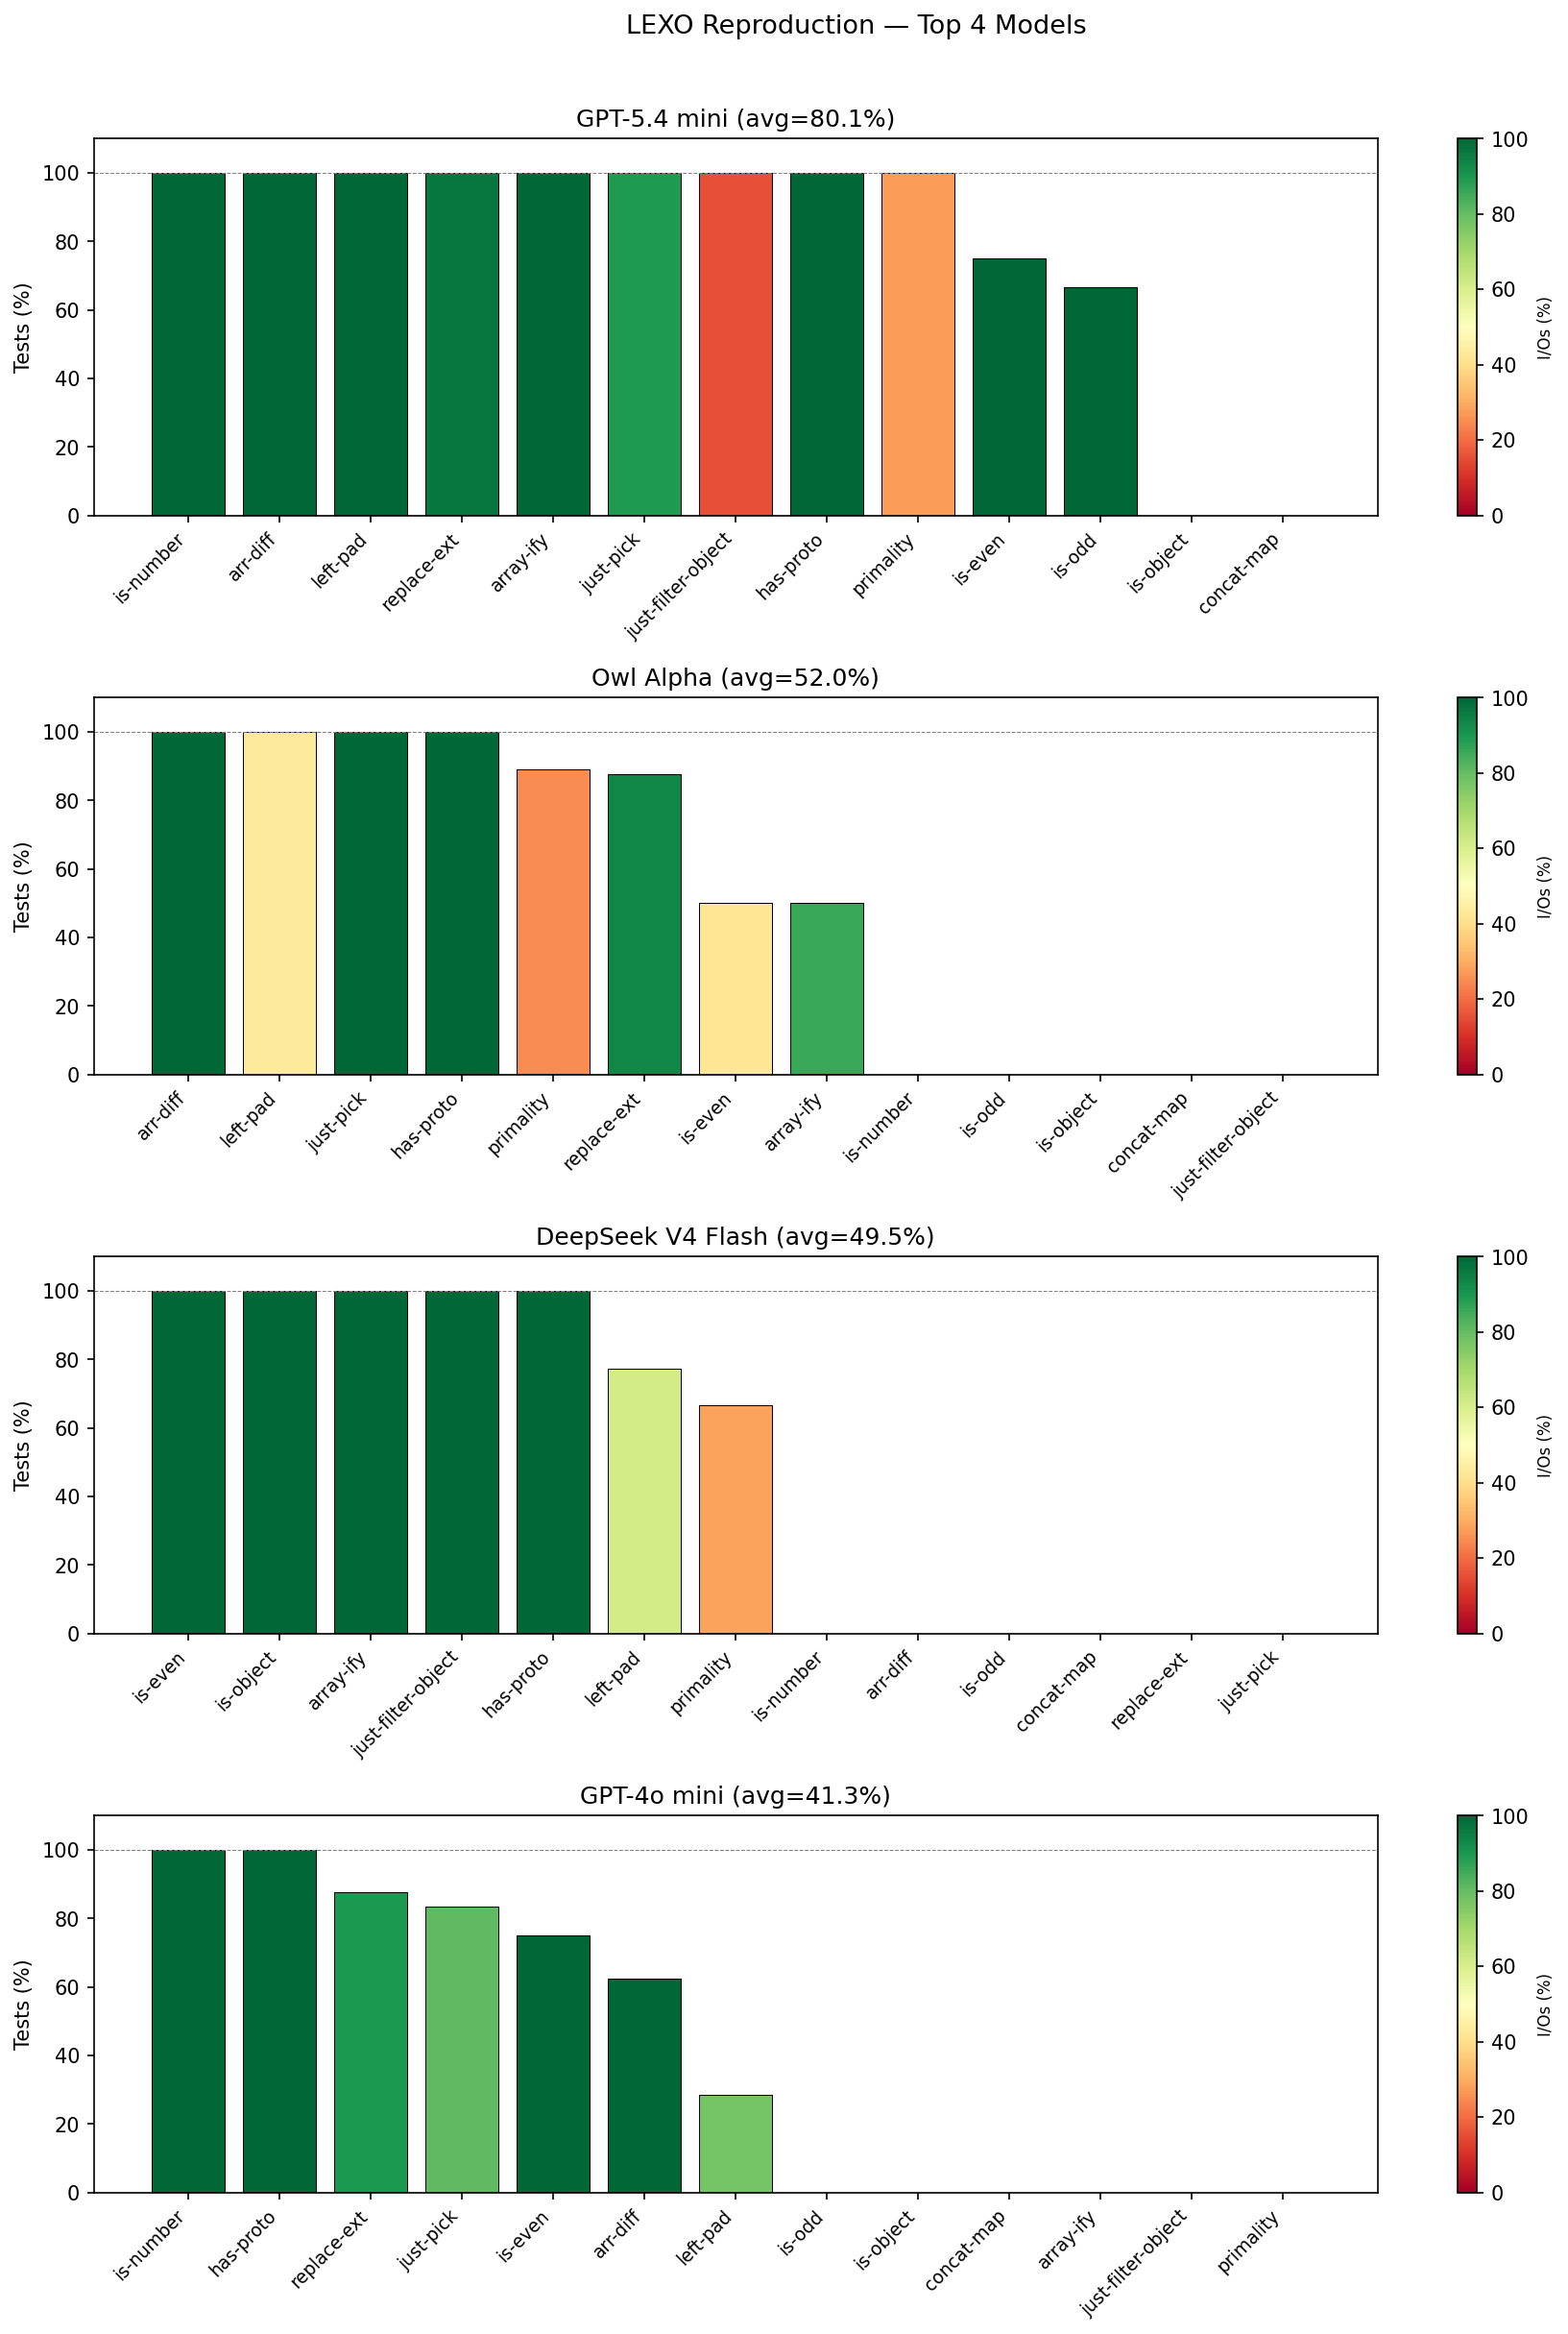
\includegraphics[width=\textwidth]{results/figure3_top4.png}
    \caption{Baseline — top 4 models by average score.}
\end{figure}

\begin{figure}[H]
    \centering
    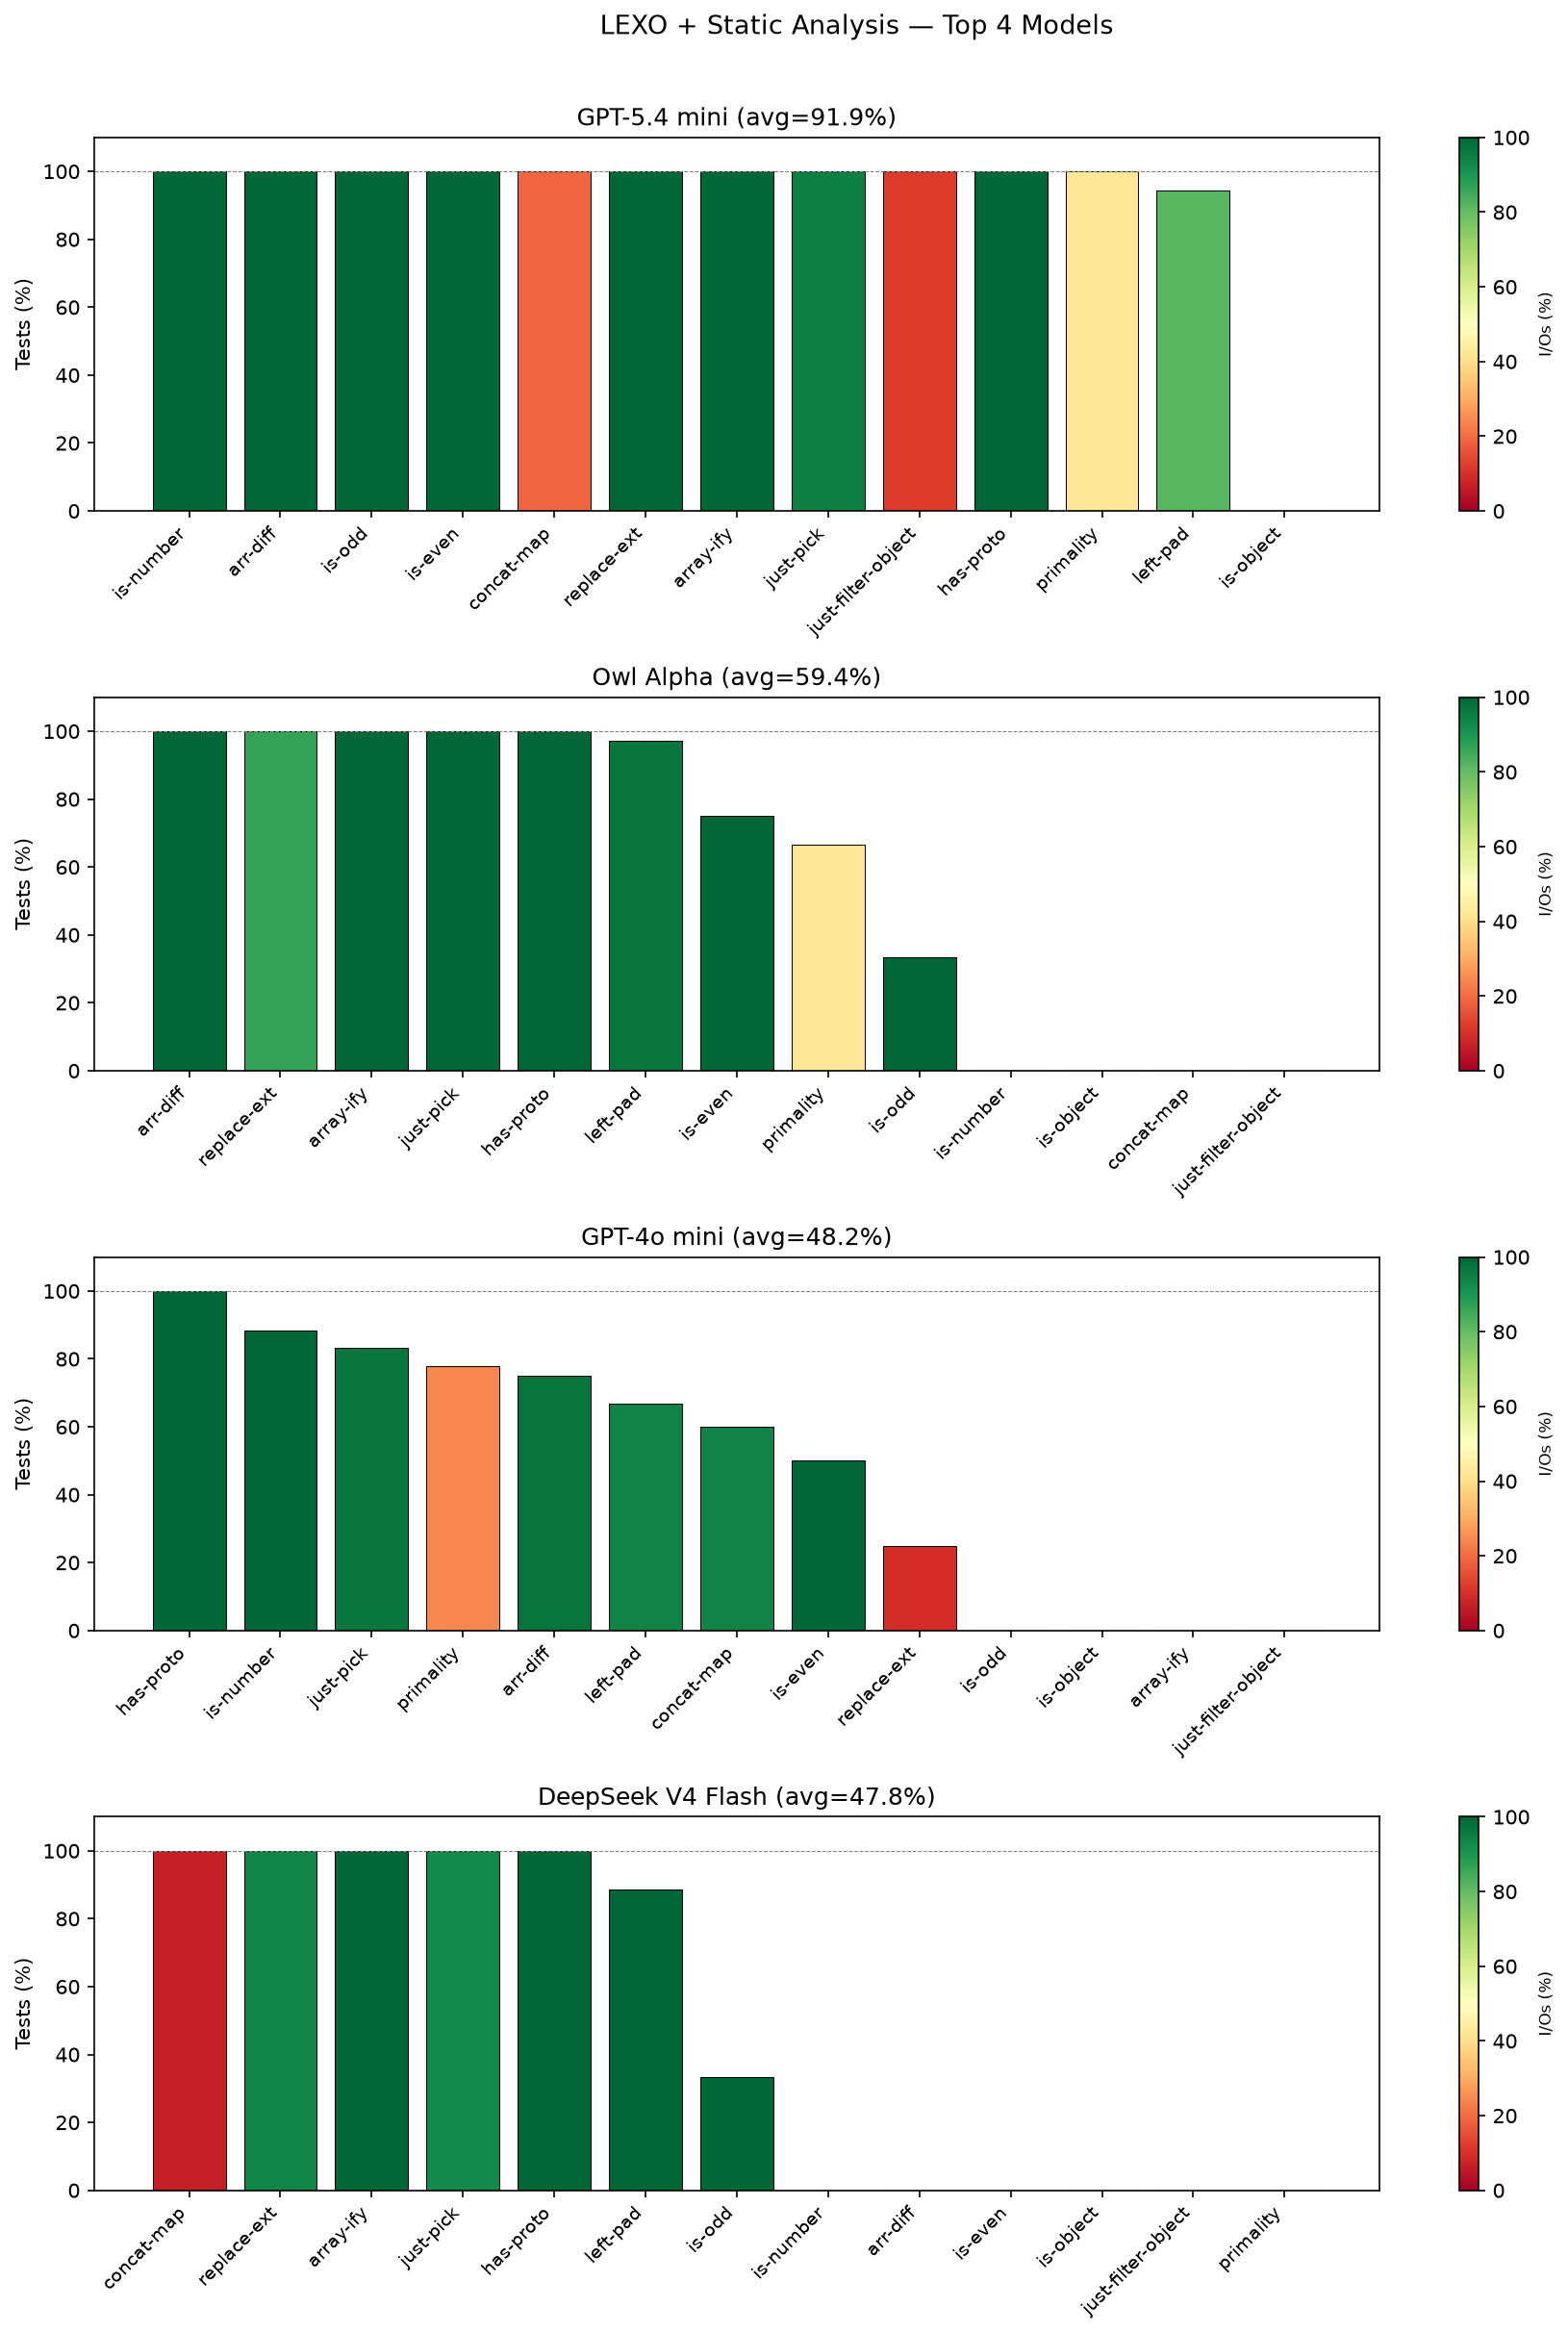
\includegraphics[width=\textwidth]{results/figure3_enriched_top4.png}
    \caption{Enrichment V1 (signatures + documentation) — top 4 models.}
\end{figure}

\begin{figure}[H]
    \centering
    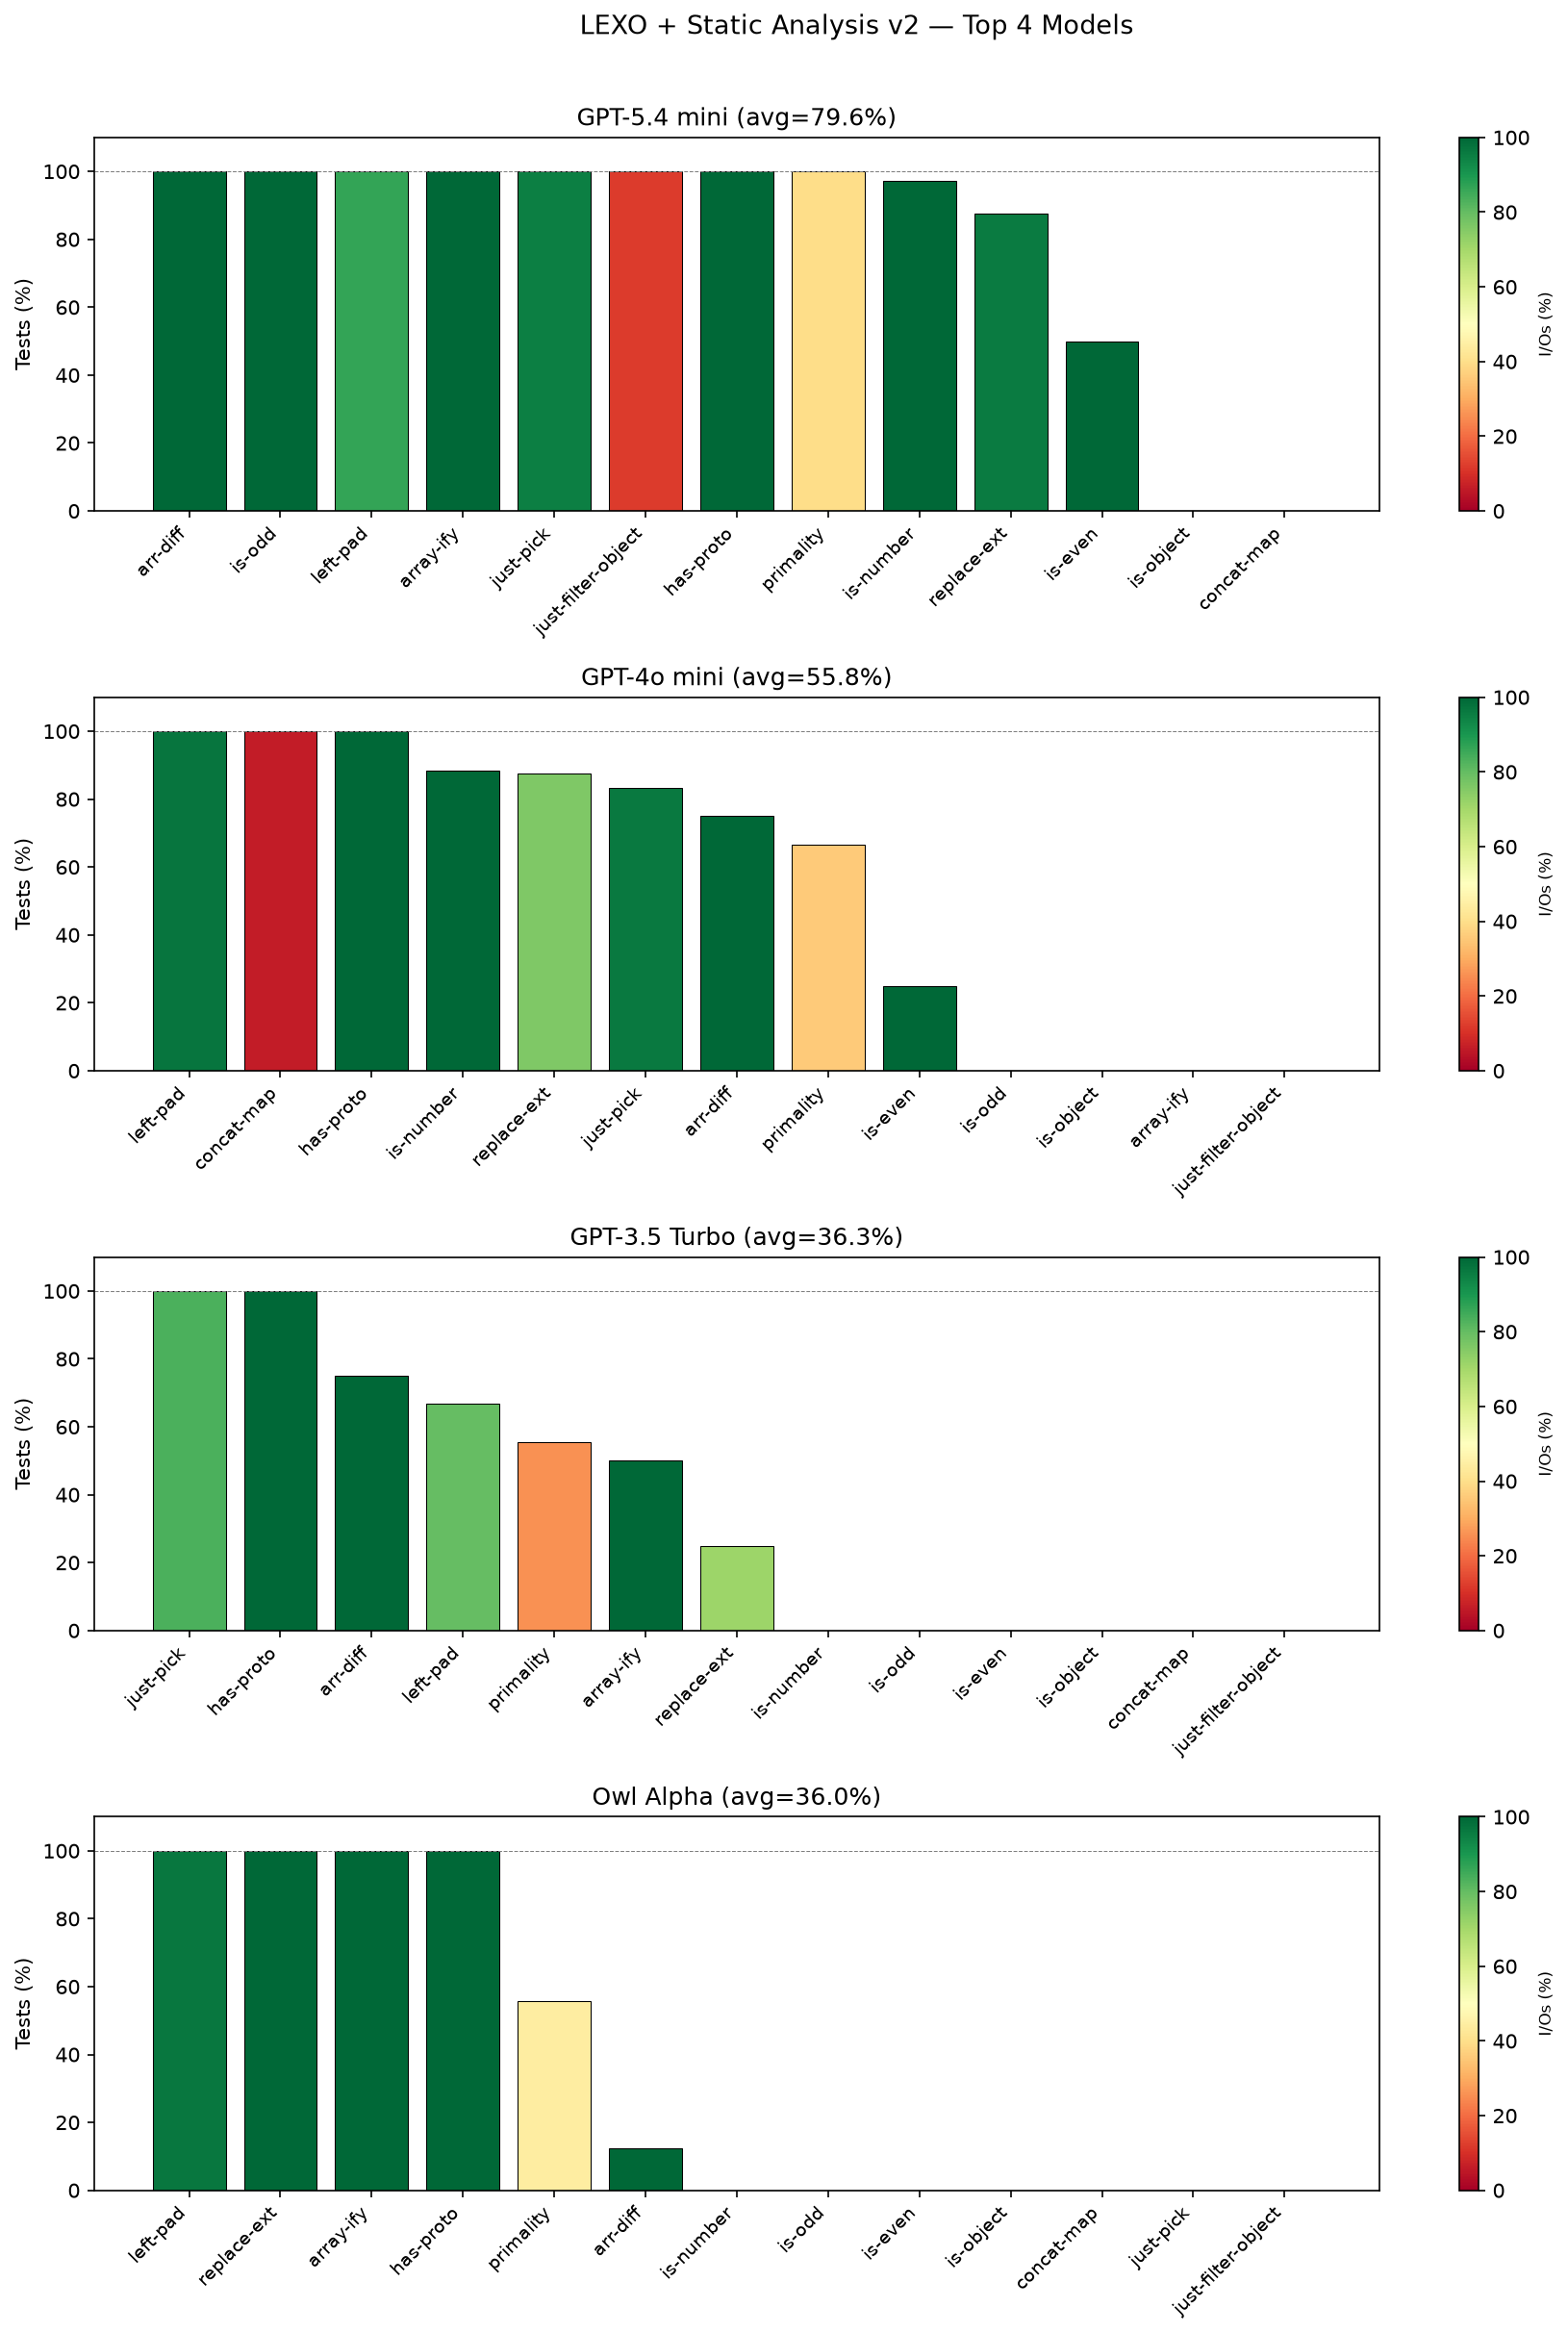
\includegraphics[width=\textwidth]{results/figure3_enriched_v2_top4.png}
    \caption{Enrichment V2 (V1 + function body) — top 4 models.}
\end{figure}

\begin{figure}[H]
    \centering
    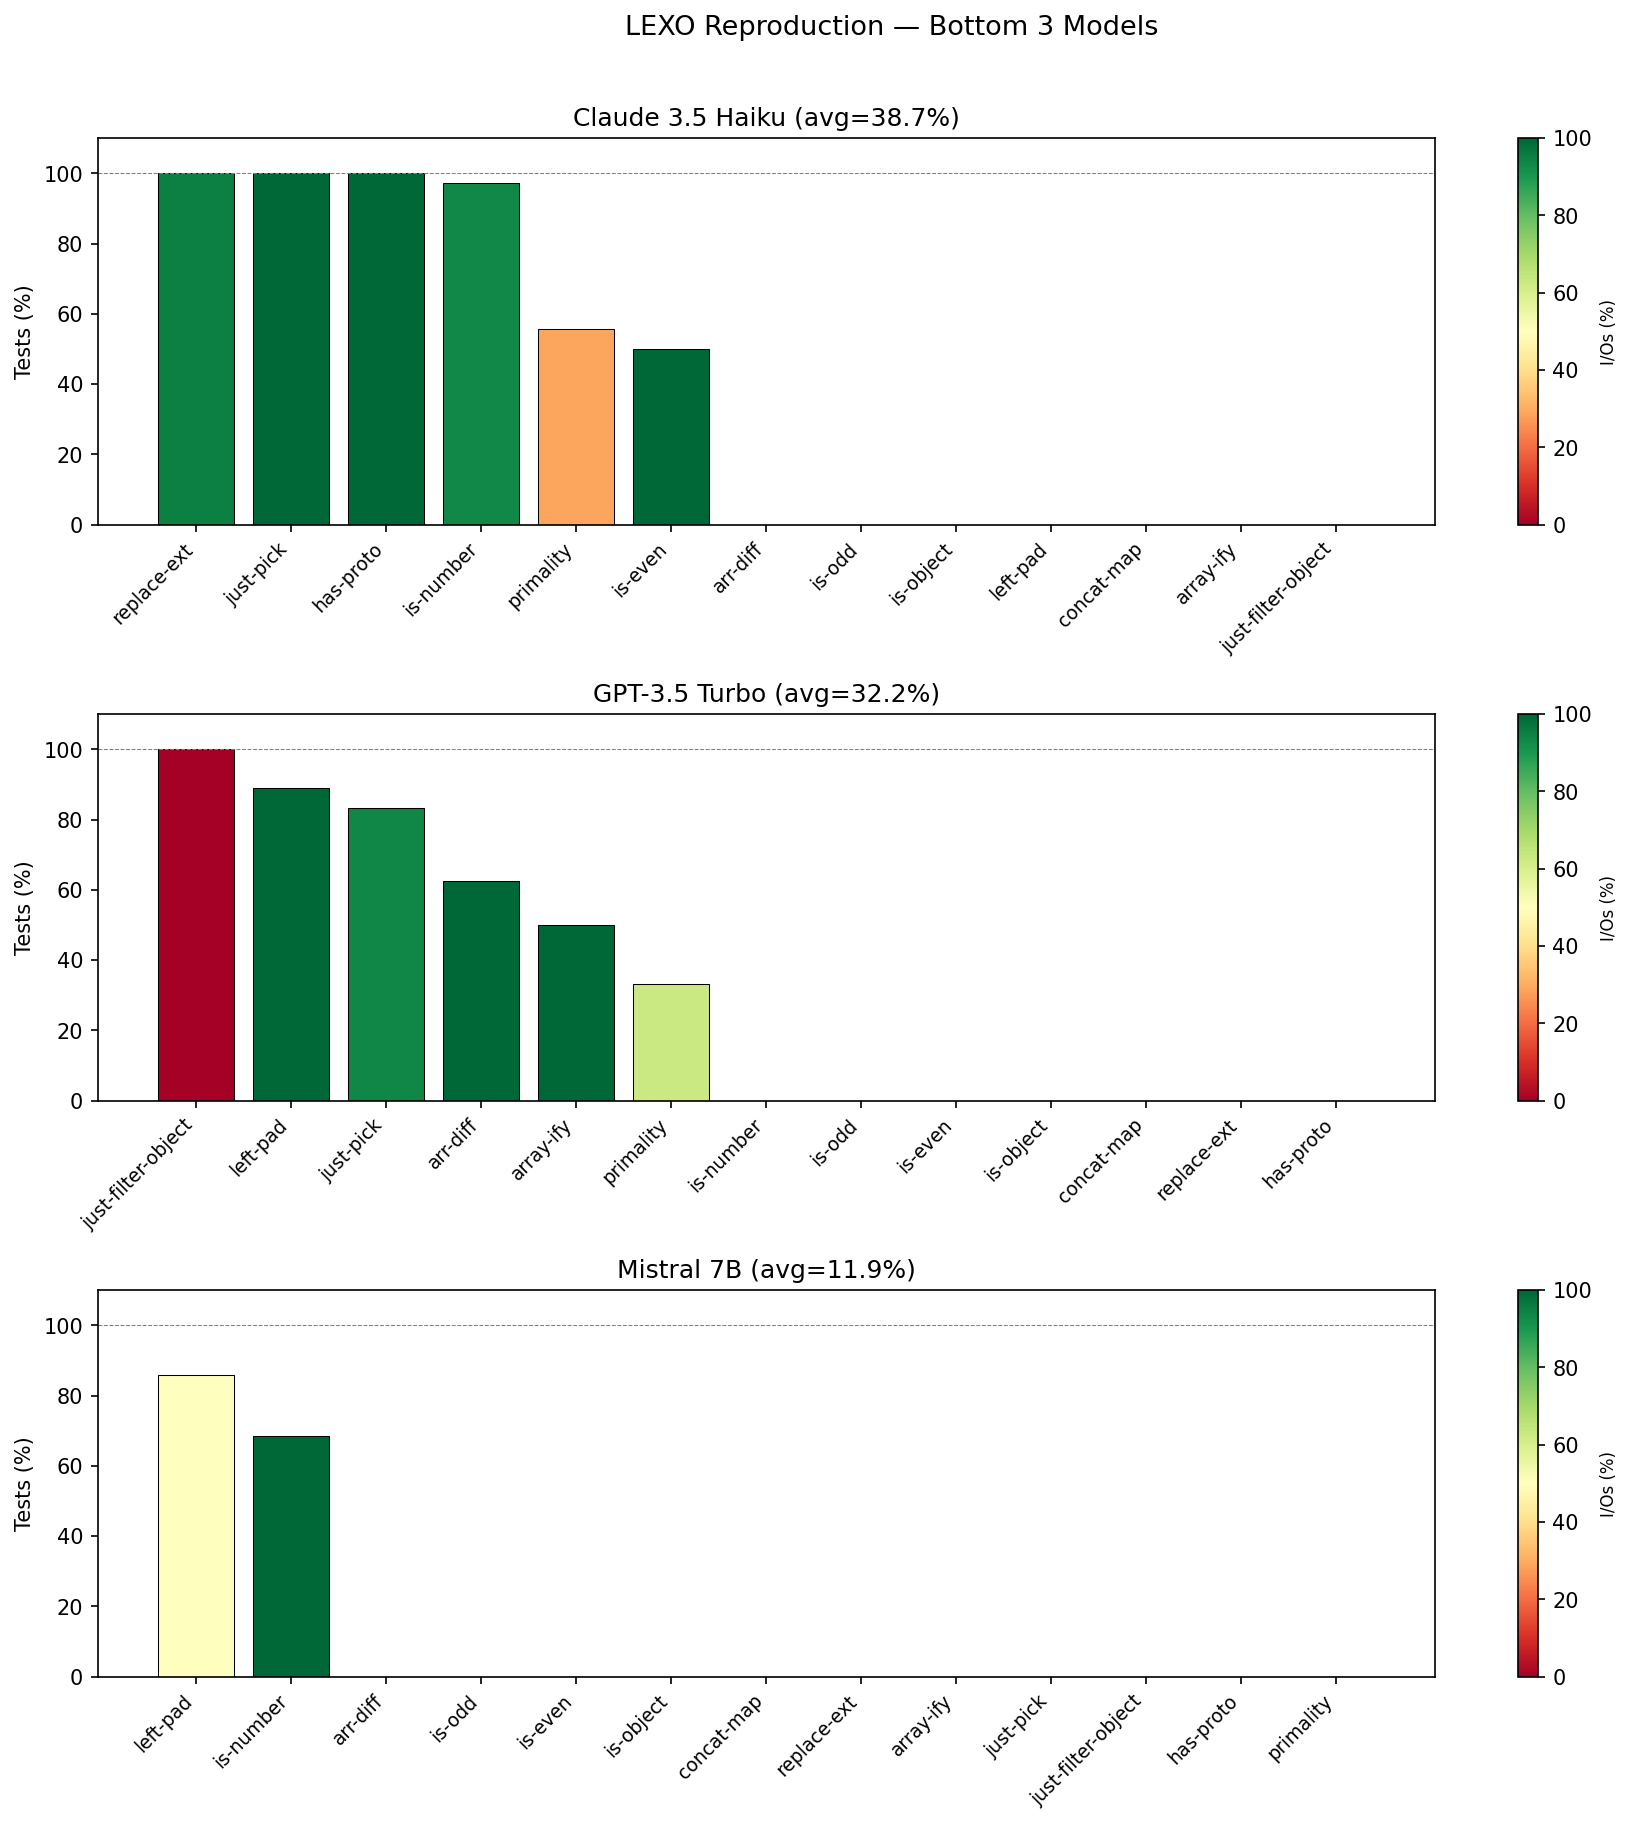
\includegraphics[width=\textwidth]{results/figure3_bottom3.png}
    \caption{Baseline — bottom 3 models.}
\end{figure}

\begin{figure}[H]
    \centering
    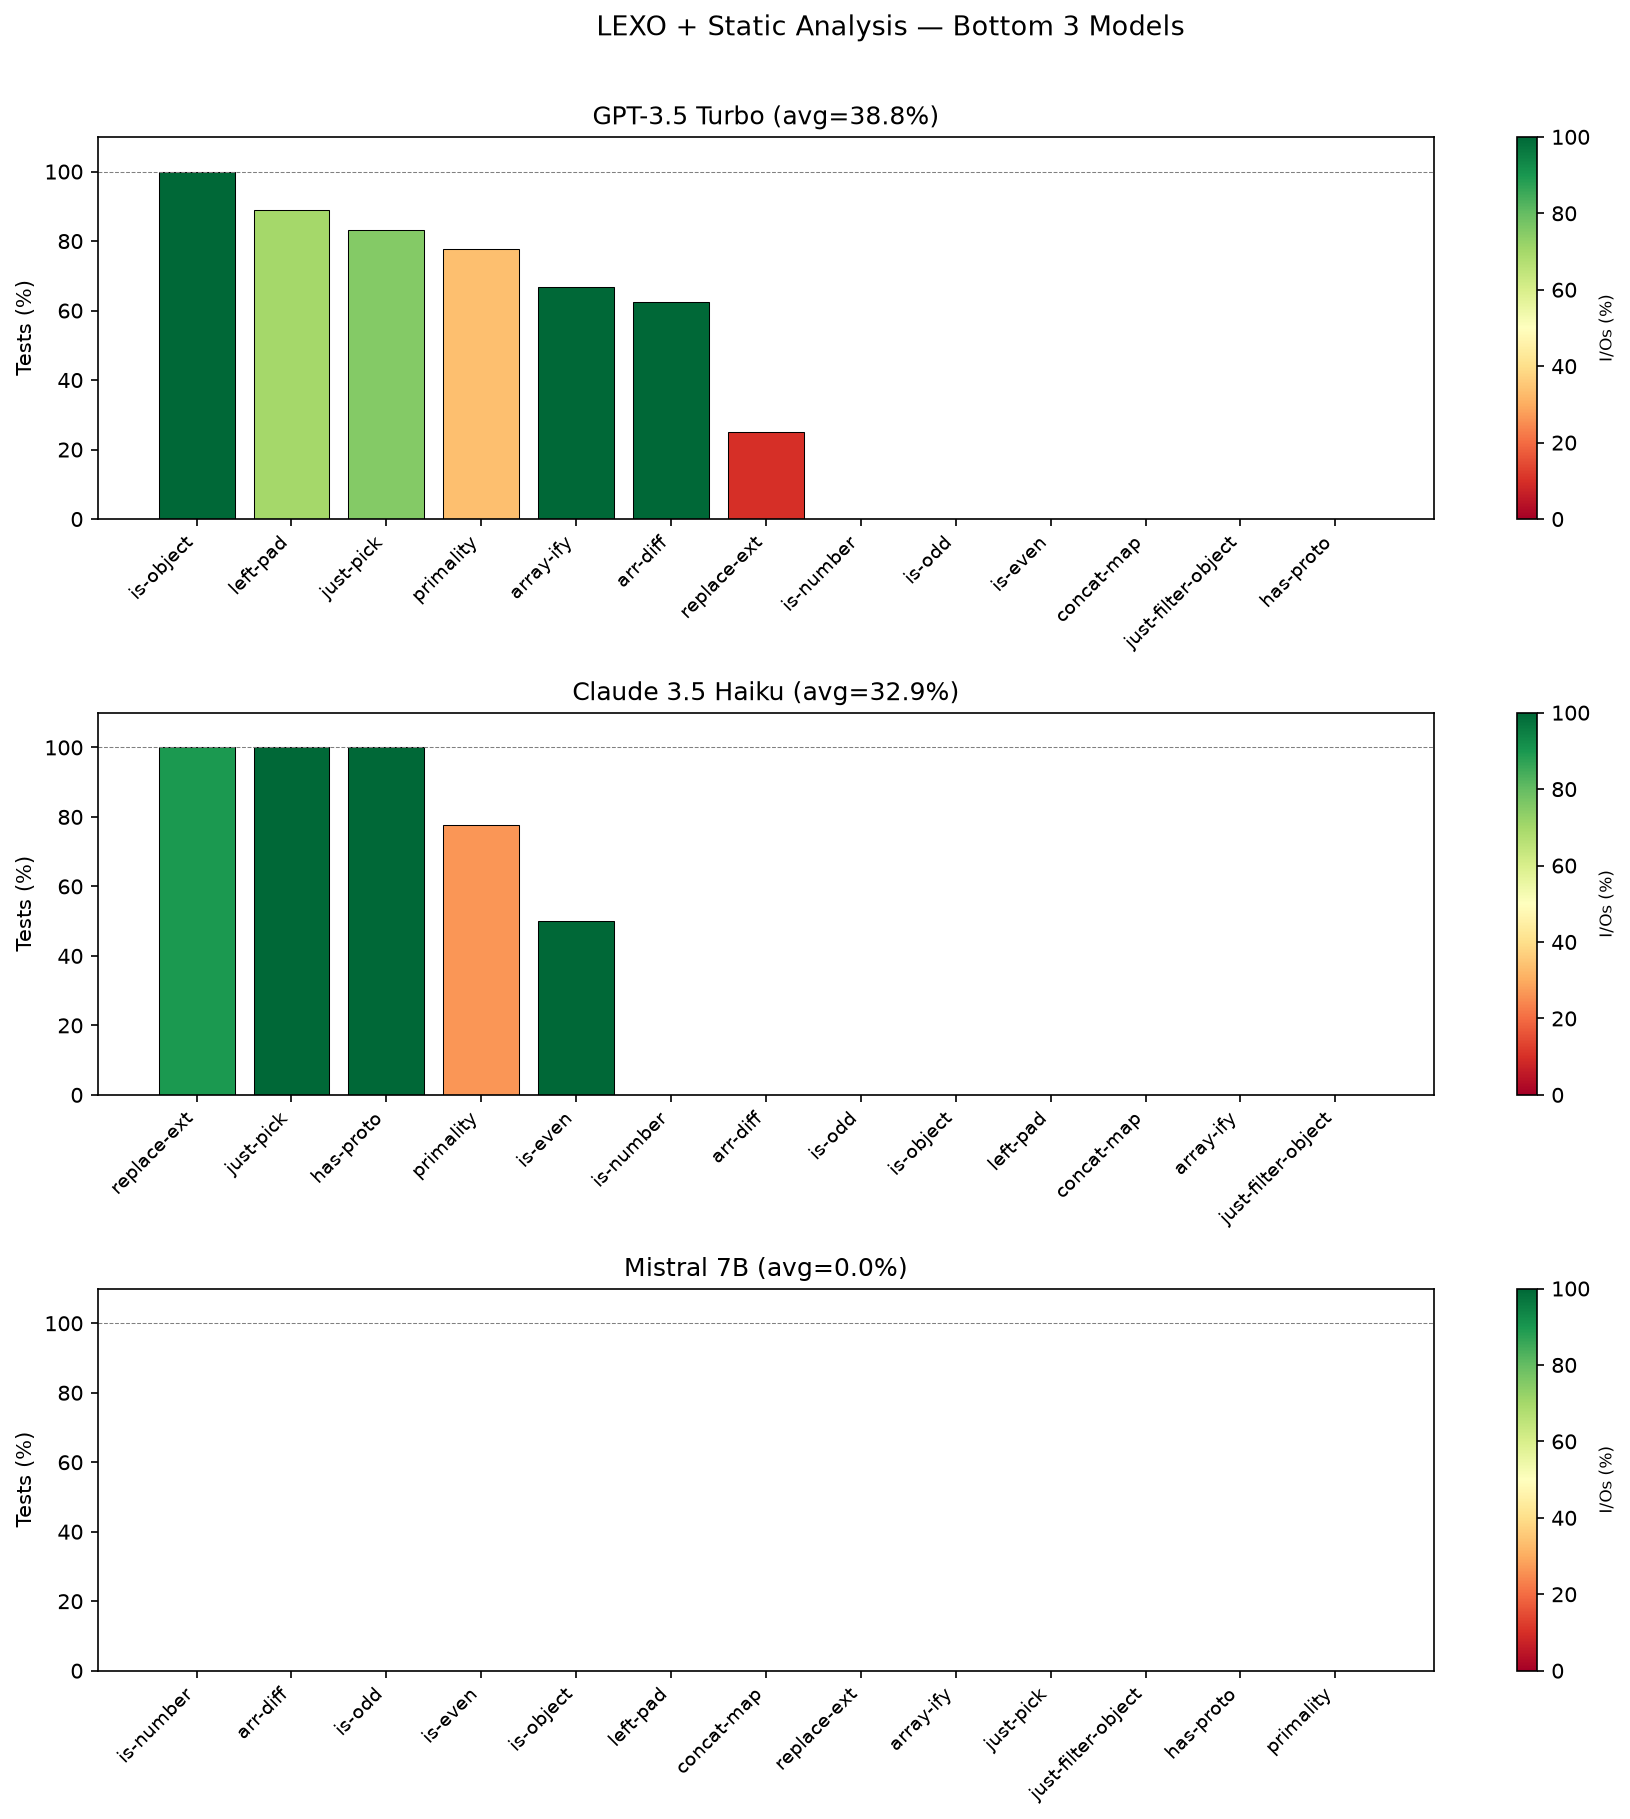
\includegraphics[width=\textwidth]{results/figure3_enriched_bottom3.png}
    \caption{Enrichment V1 — bottom 3 models.}
\end{figure}

\begin{figure}[H]
    \centering
    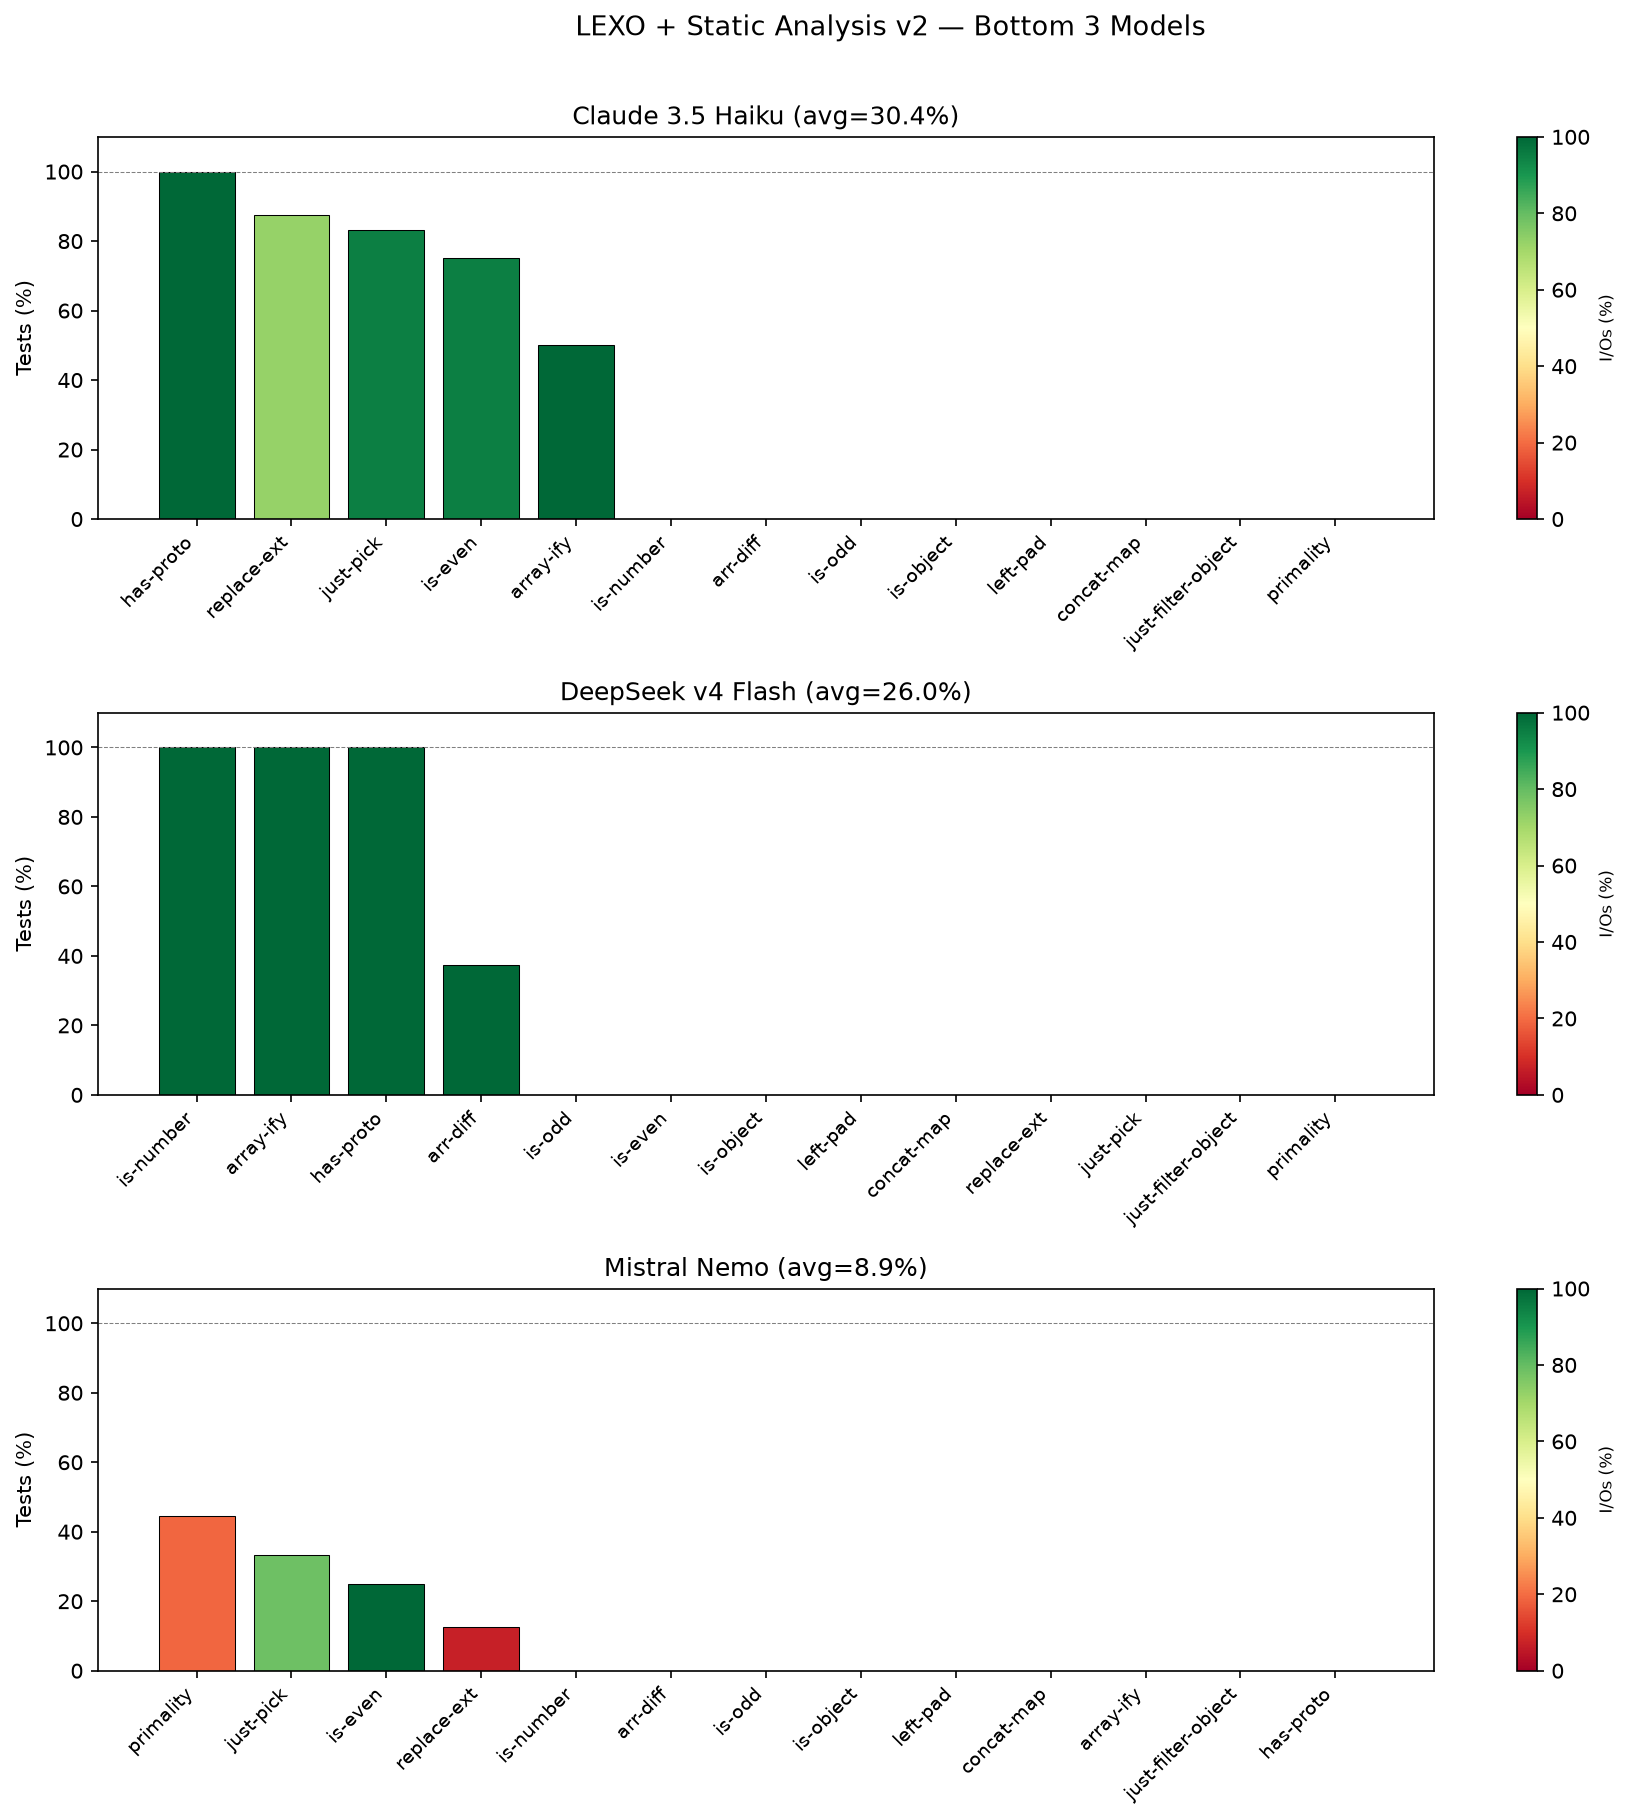
\includegraphics[width=\textwidth]{results/figure3_enriched_v2_bottom3.png}
    \caption{Enrichment V2 — bottom 3 models.}
\end{figure}

\section{Analysis}

\textbf{V1 improves stronger models.} GPT-5.4 mini (+12.7\%), DeepSeek (+8.3\%), and Claude Haiku (+1.8\%) all improved. The gains are most visible on packages with rich documentation: \texttt{primality} (Python docstrings with type annotations) improved across all capable models — GPT-4o mini from 0\% to 77.8\%, Claude Haiku from 55.6\% to 77.8\%, GPT-3.5 Turbo from 33.3\% to 77.8\%. The metadata gave the LLM explicit context about parameter types, valid ranges, and expected exceptions, resulting in more diverse and semantically grounded test inputs.

\textbf{V1 hurts weaker models.} Owl Alpha ($-$14.3\%) and Mistral Nemo ($-$6.8\%) regressed. The additional prompt length appears to increase the probability of malformed JSON output in models that already struggle with structured output. The gain in semantic grounding is outweighed by the loss in output reliability.

\textbf{V2 results are mixed.} GPT-4o mini improved further to +12.9\% overall, with notable gains on \texttt{left-pad} (28.6\% $\rightarrow$ 100\%) and \texttt{concat-map} (60\% $\rightarrow$ 100\%) — cases where seeing the implementation helped. However, error counts increased for Owl Alpha (2 $\rightarrow$ 6 errors) and DeepSeek (6 $\rightarrow$ 9 errors), indicating that the body slice increases prompt complexity beyond what these models can reliably handle.

\textbf{The \texttt{has-proto} case.} Despite the added module-level context in V2, \texttt{has-proto} still scores 100\% dev tests across all models in all three runs. This is because the function genuinely always returns \texttt{true} in any modern JS engine — the IIFE computes a boolean at module load time that is always \texttt{true} in V8. The regenerated \texttt{return true} is actually correct. The overfitting problem exists but is invisible to the dev test metric in this specific case.

\section{Conclusion}

Static analysis enrichment is a lightweight, zero-cost addition to the LEXO pipeline. V1 (signatures + documentation) is the more robust improvement, consistently helping capable models while being transparent about its limitations on undocumented packages. V2 (adding function body) shows selective gains but increases prompt complexity with diminishing returns for most models.

The results confirm that the quality of I/O pair generation is a significant driver of final correctness. Providing structured semantic context improves input diversity, particularly for packages with rich documentation. For undocumented packages, the metadata is too sparse to be impactful — a finding that points toward alternative enrichment strategies such as type inference or documentation generation as preprocessing steps.

\bigskip
\noindent\textbf{Repository:} \url{https://github.com/Abdelhak-Chellal/Lexo-repro}

\end{document}
